\documentclass[border=10pt]{standalone}

\usepackage{tikz}
\usepackage{tikzsymbols}
\usetikzlibrary{calc,patterns,shapes.geometric}

\def\centerarc[#1](#2)(#3:#4:#5){\draw[#1] ($(#2)+({#5*cos(#3)},{#5*sin(#3)})$) arc (#3:#4:#5);}

\begin{document}
	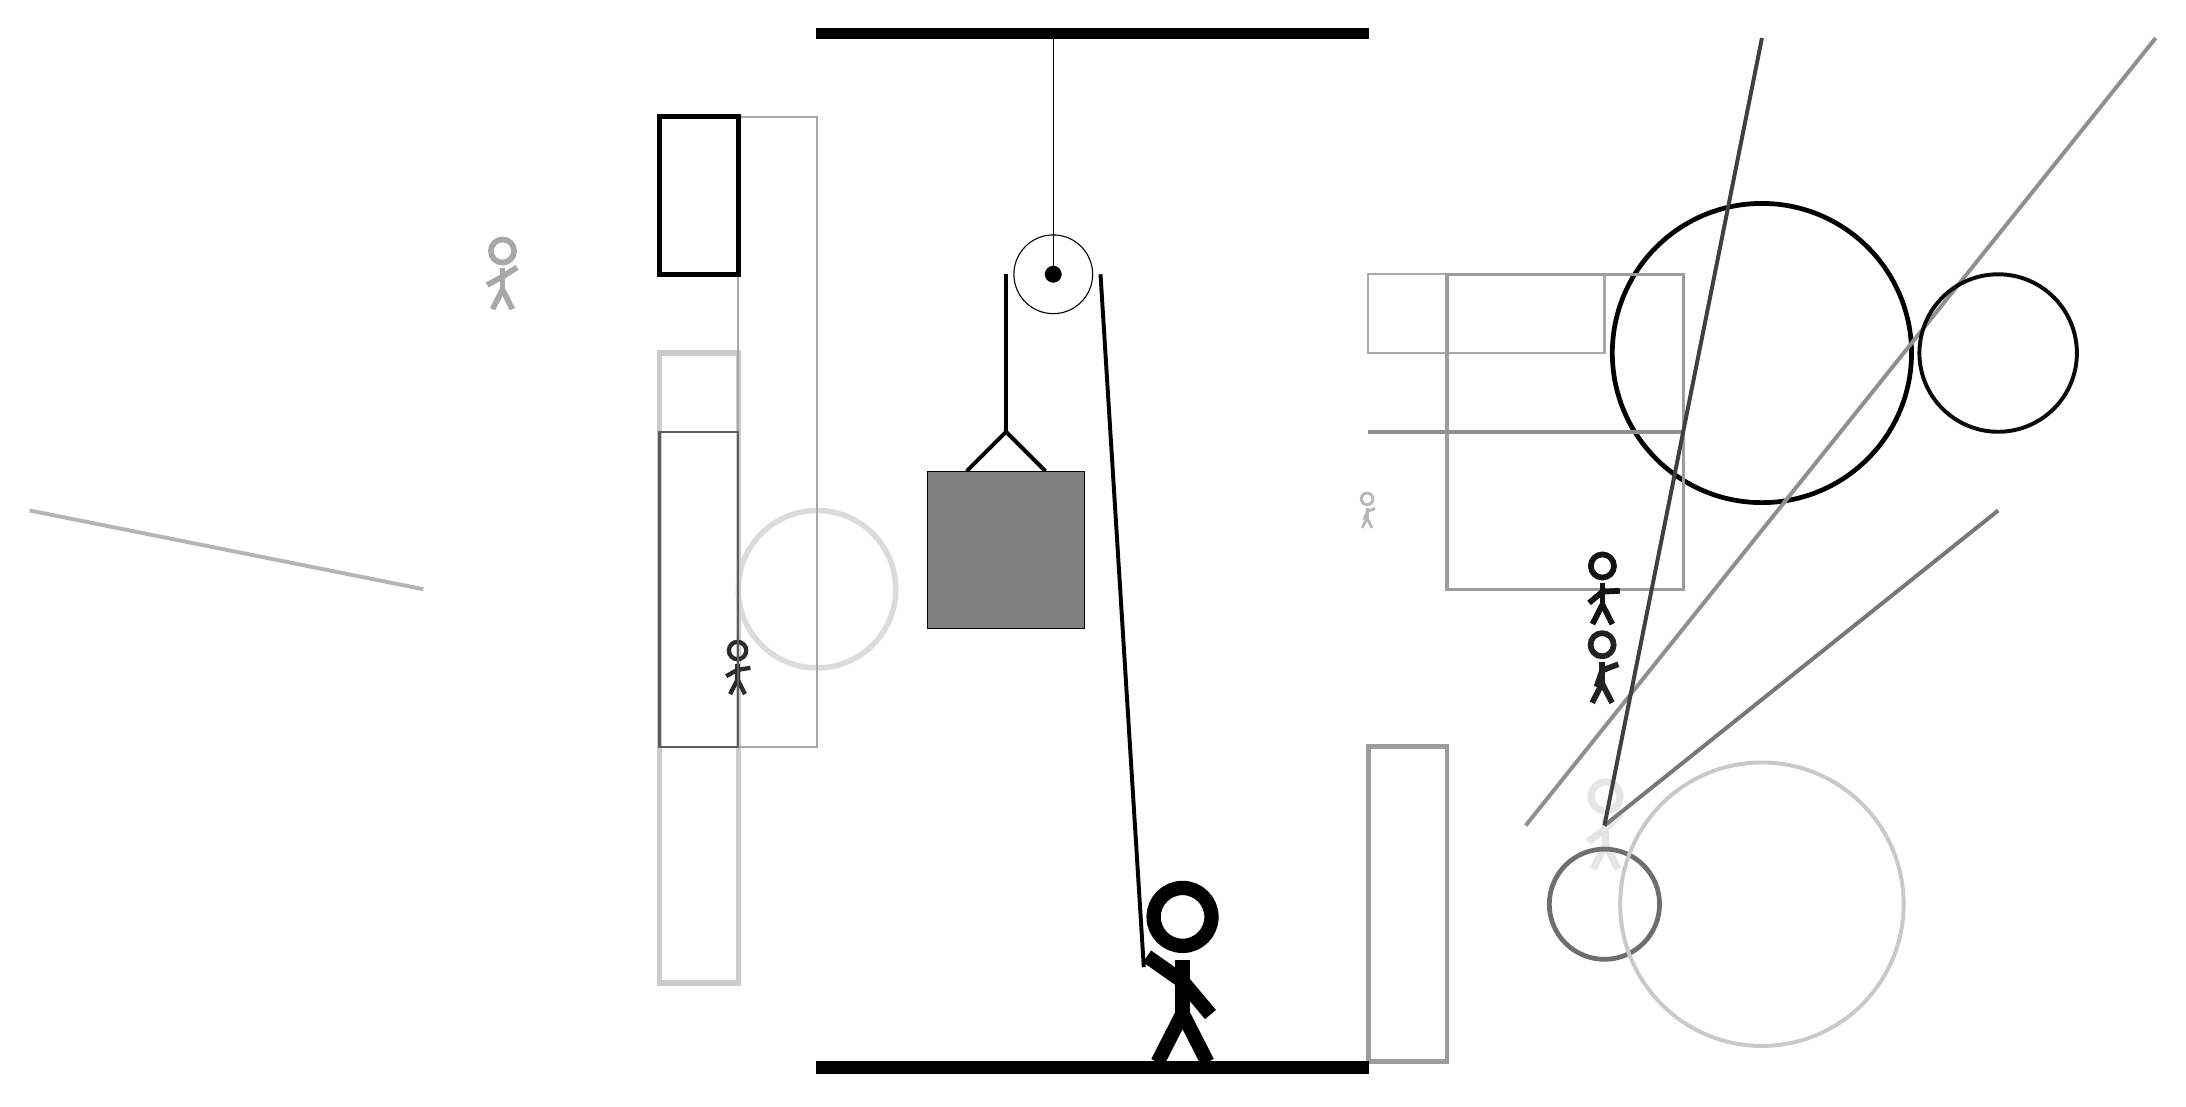
\begin{tikzpicture}
		%%%%% START %%%%%
		
		\draw[fill=black] (-2, 10) rectangle (5, 10.125);
		
		\draw (1, 7) circle (0.5);
		\draw[fill=black] (1, 7) circle (0.1);
		\draw (1, 10) -- (1, 7);
		
		\draw[line width=0.5mm] (-0.1, 4.5) -- (0.4, 5.0) -- (0.9, 4.5);
		\draw[fill=black!50] (-0.6, 4.5) rectangle (1.4, 2.5);
		
		\draw[line width=0.5mm] (0.4, 7) -- (0.4, 5.0);
		\centerarc[line width=0.5mm](1, 7)(0:180:0.6);
		\draw[line width=0.5mm](1.6, 7) -- (2.15, -1.8);
		
		\node at (2.6, -1.9) {\Strichmaxerl[10][-35][-50]};
		
		\draw [line width=0.7mm, color=black!14](-2, 3) circle (1.0);
		
		\draw [line width=0.6mm, color=black!100](10, 6) circle (1.9);
		\node[line width=0.2mm, color=black!10] at (8, 0) {\Strichmaxerl[5][37][46]};
		\draw[line width=0.5mm, color=black!44](7, 0) -- (15, 10);
		
		\node[line width=0.2mm, color=black!34] at (-6, 7) {\Strichmaxerl[4][28][33]};
		\draw [line width=0.6mm, color=black!57](8, -1) circle (0.7);
		\draw[line width=0.3mm, color=black!34] (5, 6) rectangle (8, 7);
		\draw[line width=0.7mm, color=black!20] (-4, 6) rectangle (-3, -2);
		\draw[line width=0.3mm, color=black!34] (-3, 1) rectangle (-2, 9);
		\draw[line width=0.4mm, color=black!39] (6, 7) rectangle (9, 3);
		
		\draw[line width=0.5mm, color=black!53](8, 0) -- (13, 4);
		\node[line width=0.7mm, color=black!83] at (-3, 2) {\Strichmaxerl[3][29][9]};
		\node[line width=0.4mm, color=black!28] at (5, 4) {\Strichmaxerl[2][68][23]};
		
		\draw[line width=0.5mm, color=black!29](-7, 3) -- (-12, 4);
		\node[line width=0.3mm, color=black!87] at (8, 2) {\Strichmaxerl[4][71][21]};
		\draw[line width=0.3mm, color=black!64] (-3, 5) rectangle (-4, 1);
		
		\draw [line width=0.5mm, color=black!96](13, 6) circle (1.0);
		
		\node[line width=0.4mm, color=black!93] at (8, 3) {\Strichmaxerl[4][40][3]};
		\draw[line width=0.6mm, color=black!100] (-4, 7) rectangle (-3, 9);
		
		\draw [line width=0.5mm, color=black!21](10, -1) circle (1.8);
		\draw[line width=0.5mm, color=black!44](9, 5) -- (5, 5);
		\draw[line width=0.5mm, color=black!75](8, 0) -- (10, 10);
		\draw[line width=0.6mm, color=black!39] (6, -3) rectangle (5, 1);
		
		\draw[fill=black] (-2, -3) rectangle (5, -3.15);
		
		%%%%% END %%%%%
	\end{tikzpicture}
\end{document}